\section{Effets :}
\emph{Interface :}

L'utilisateur choisit un effet parmi la liste d'effets affichée en bas de l'écran, ce qui affiche les 
réglages disponibles (s'il y en a). L'utilisateur peut ensuite choisir de confirmer ou d'annuler la modification
apportée par l'effet choisi.
\\

\emph{Structure du code :}

Les effets sont rassemblés dans le package filters (fr.ubordeaux.pimp.filters).
La classe \emph{Retouching} contient les réglages de luminosité, contraste, saturation et teinte.
La classe \emph{Convolution} contient tous les effets liés à la convolution (flou, détection de contour etc.).
Toutes ces méthodes sont appelées lors de l'appui de boutons ou de glissement de seekbars. Les seekbars ont généralement
une étendue allant de 0 à 255 (sauf pour les réglages de teinte), et certains effets nécessitent des valeurs pouvant être
négatives. Ainsi la valeur de seekbar est modifiée dans la méthode appelante de ces mêmes effets.

Tous les effets nécessitant l'histogramme utilise celui de la \emph{valeur}, soit le maximum entre les trois canaux RGB.

\subsection{Luminosité (Brightness) :}
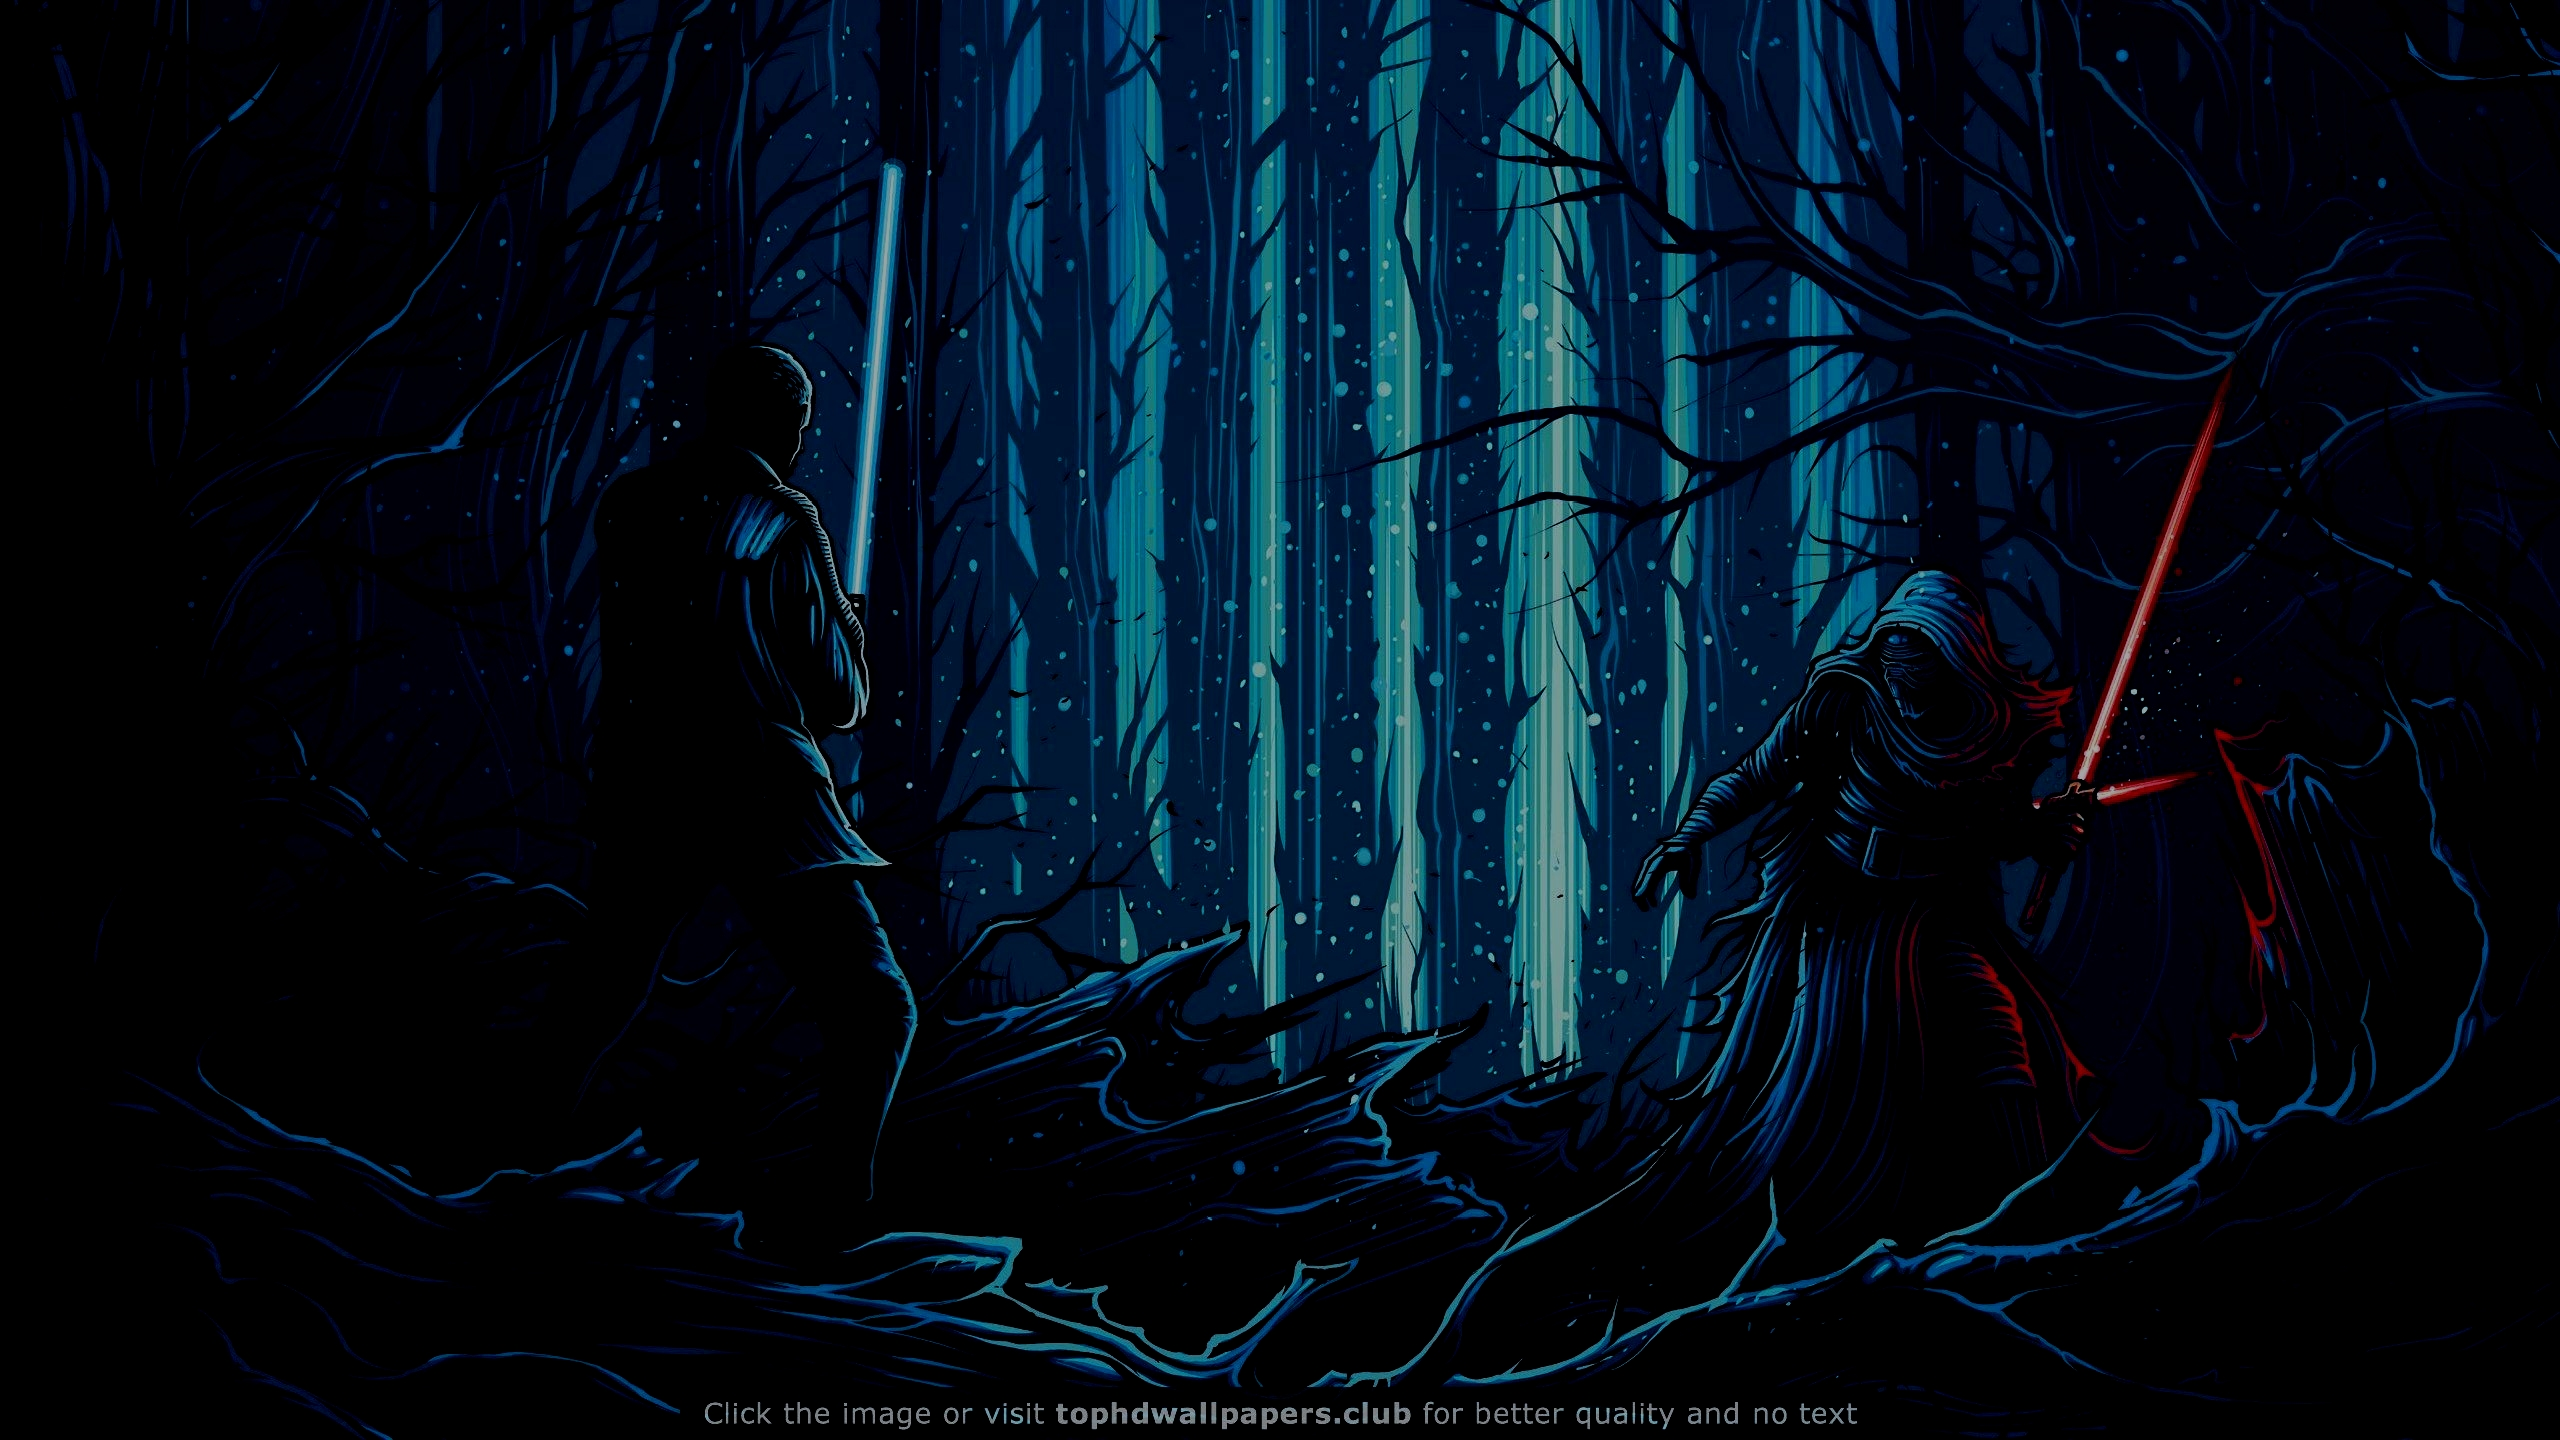
\includegraphics[width=0.5\textwidth]{report_src/brightness_low.jpeg}
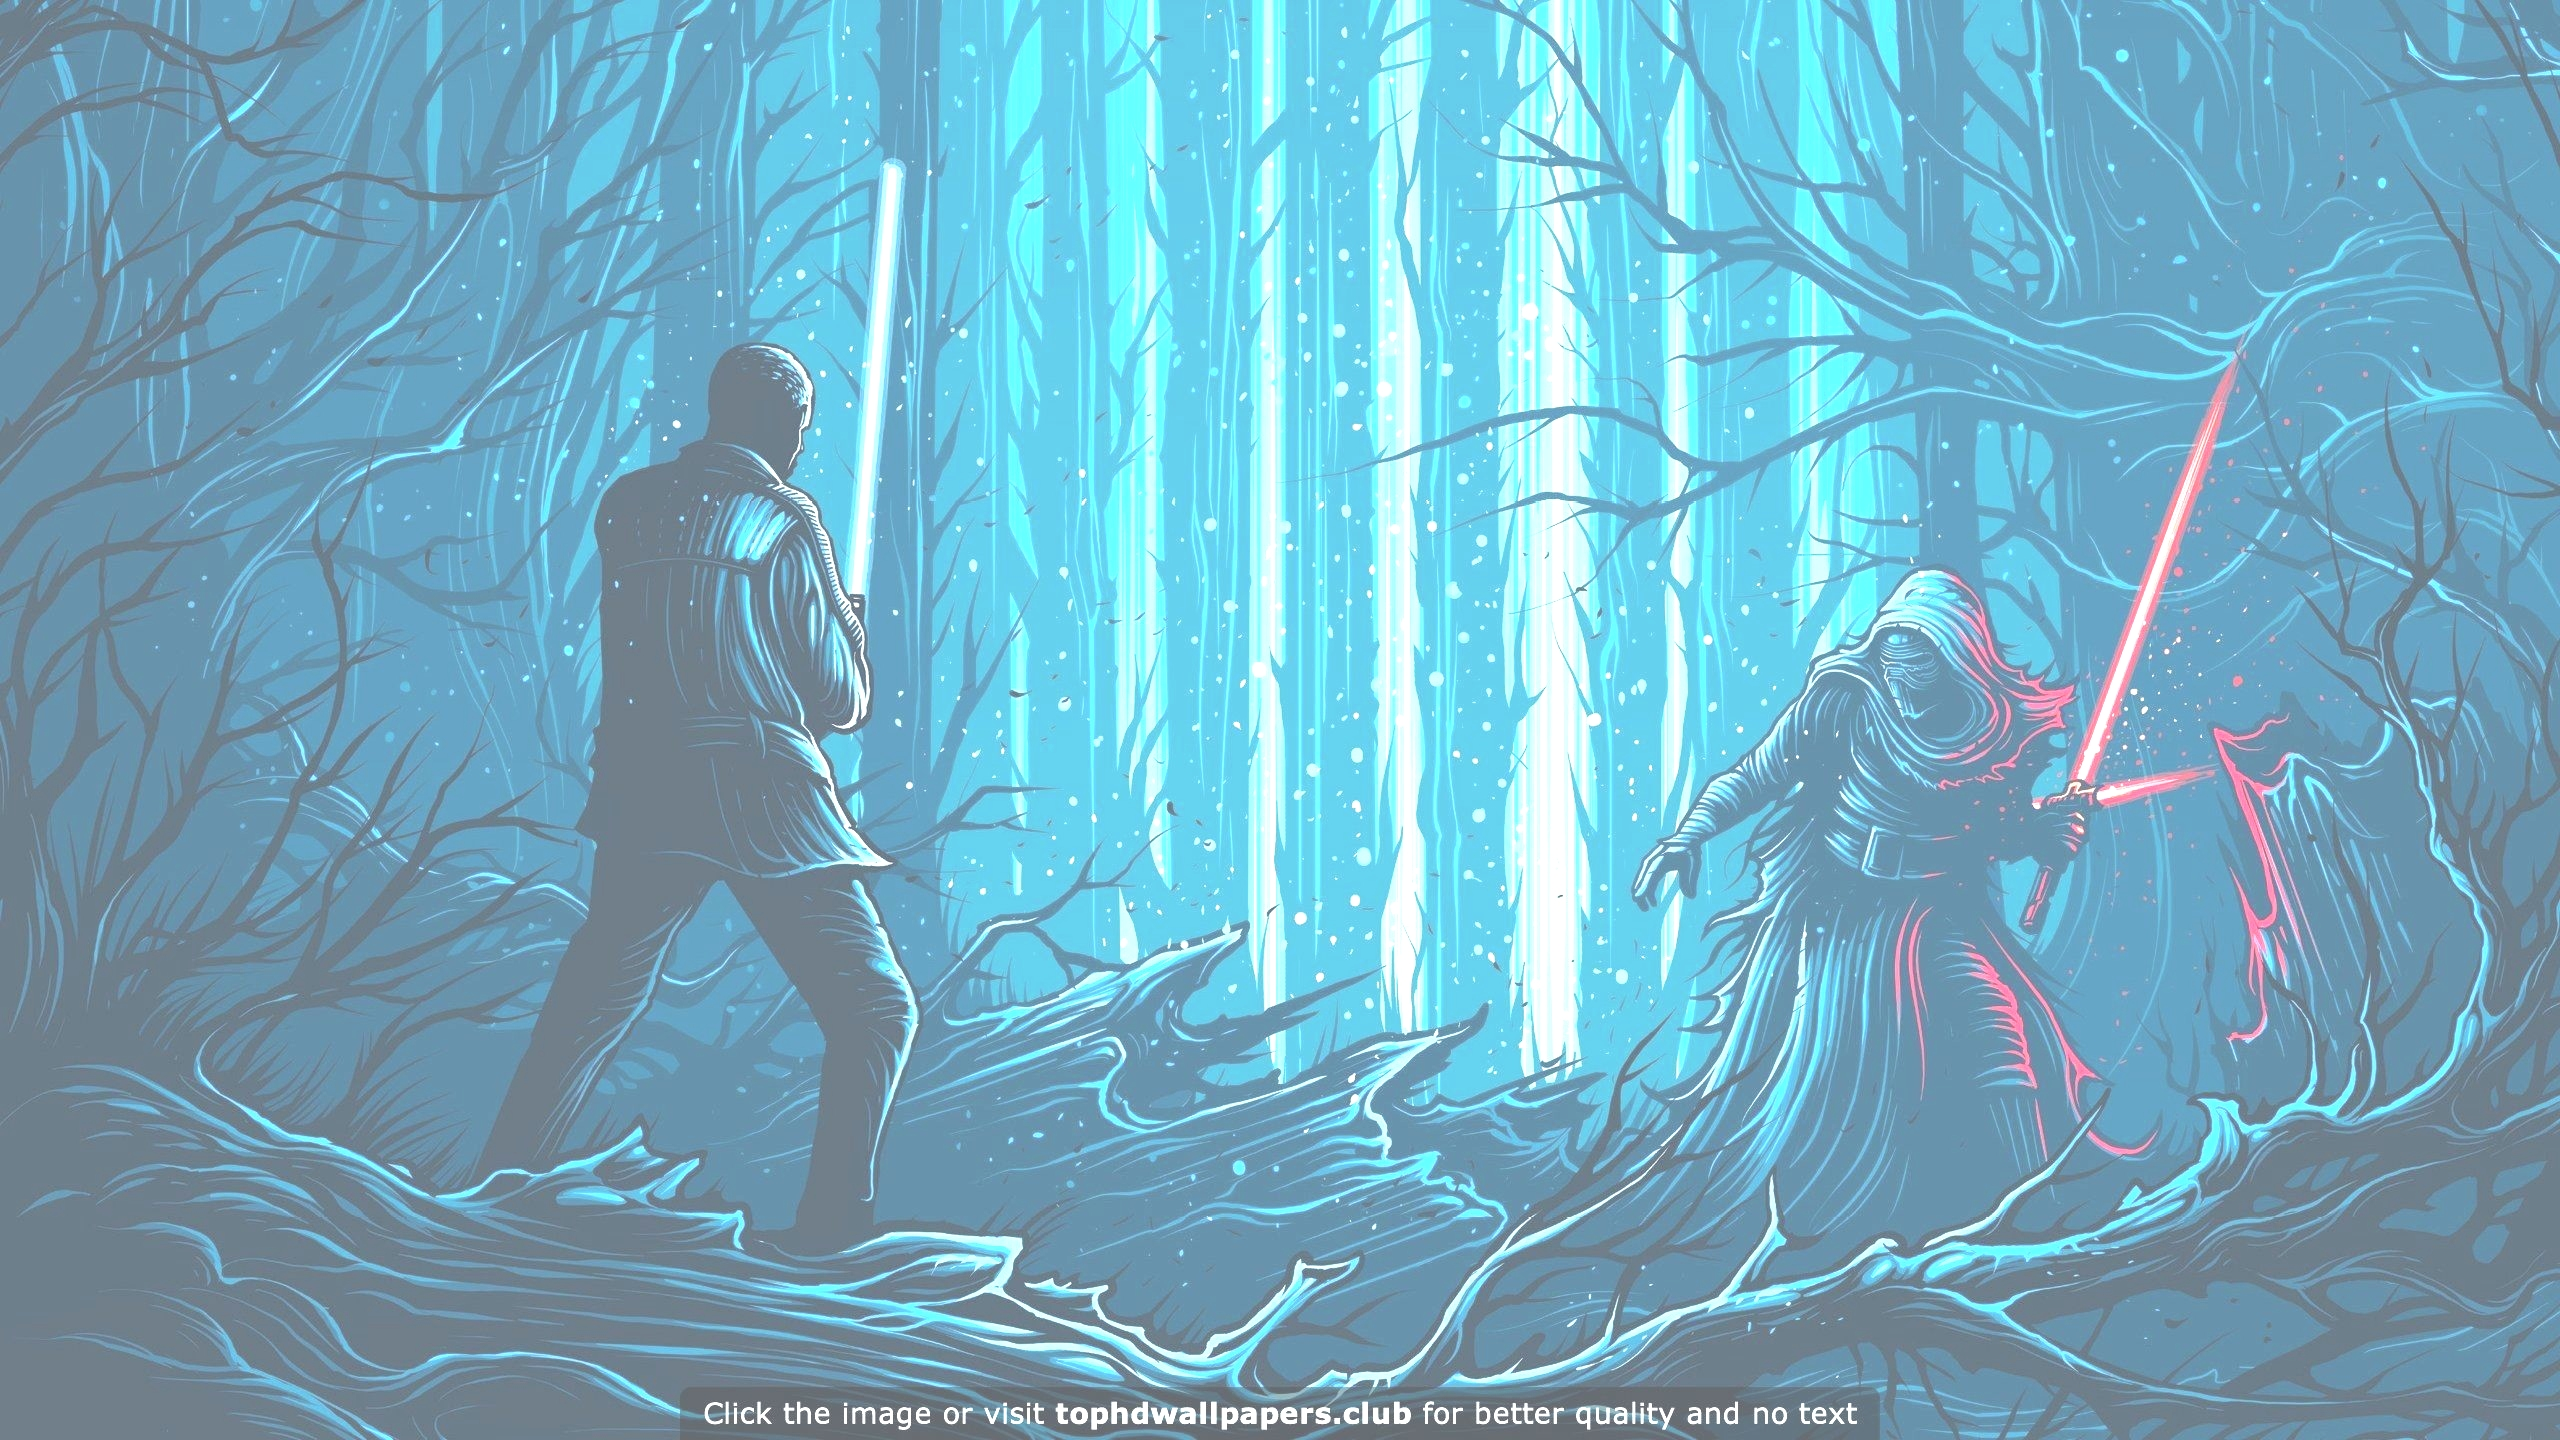
\includegraphics[width=0.5\textwidth]{report_src/brightness_high.jpeg}

\emph{Méthode appelante : Retouching.setBrightness()}

\emph{Script : brightness.rs}
\\

Ce réglage ajoute une valeur (positive ou négative) aux trois canaux RGB de l'image. Cette valeur est fixée par la seekbar.
Les valeurs sont tronquées entre 0 et 255, par conséquent on perd de l'information dans les valeurs extrêmes de luminosité.

Cet effet n'utilise pas la luminosité existante de l'image, ainsi on peut obtenir des résultats qui sont parfois discutables, par exemple
le noir qui s'éclaircit et inversement pour le blanc. Pour pallier à ce problème, on pourrait introduire une multiplication afin de modifier
la luminosité proportionnellement à celle existante. Cependant, cette solution modifie aussi le contraste, nous avons donc choisi
de laisser l'algorithme tel quel.


\subsection{Contraste (Contrast) :}

\emph{Méthode appelante : Retouching.dynamicExtensionRGB()}

\emph{Script : dynamicExtension.rs}
\\

Ce réglage effectue une extension linéaire de dynamique. Les nouveaux extremum de l'histogramme sont définis à partir de la position de la seekbar.
La dynamique est ainsi étendue autour d'une valeur se situant au milieu des deux anciens extremum de l'histogramme*. On a donc une image uniforme lorsque
l'on règle le contraste au minimum. En augmentant le contraste, les extremum peuvent sortir de l'intervalle [0;255], ce qui provoque une distorsion de l'image.
\\

*Il serait peut-être plus judicieux de prendre la médiane de l'histogramme cumulé afin d'avoir une valeur qui représente mieux la "valeur moyenne" de l'image.


\subsection{Saturation (Saturation) :}

\emph{Méthode appelante : Retouching.setSaturation()}

\emph{Script : saturation.rs}
\\

Ce réglage permet de régler la saturation de l'image. Soit S la saturation existante, S' la nouvelle saturation et F le facteur de saturation. S et S' vont de 0 à 1.

On a S' = S + F * (1 - S) * S. 

On observe que la nouvelle saturation est proportionnelle à deux facteurs : l'espace restant avant une saturation totale (1-S) et la saturation existante S.
Par conséquent, en augmentant la saturation, chaque pixel tend vers sa saturation maximale, tout en garantissant une saturation proportionnelle à celle existante, évitant ainsi de saturer le gris.

\subsection{Egalisation d'histogramme (Enhance) :}

\emph{Méthode appelante : Retouching.histogramEqualization()}

\emph{Scripts : cumulativeHistogram.rs, assignLut.rs} 
\\

Comme son nom l'indique, cet effet utilise l'égalisation d'histogramme afin d'améliorer le contraste.
On calcule d'abord l'histogramme cumulé et on en déduit la LUT (Look Up Table), que nous assignons ensuite à chaque pixel.
\\

Cependant, afin d'égaliser l'histogramme, l'algorithme éclaircit les zones sombres, ce qui donne un résultat peu convaincant sur les images de faible luminosité.
Une solution à ce problème est l'égalisation d'histogramme adaptative (CLAHE), mais nous n'avons pas eu le temps de l'implémenter pour ce rendu.

